% Options for packages loaded elsewhere
\PassOptionsToPackage{unicode}{hyperref}
\PassOptionsToPackage{hyphens}{url}
\PassOptionsToPackage{dvipsnames,svgnames*,x11names*}{xcolor}
%
\documentclass[
  11pt,
]{krantz}
\usepackage{amsmath,amssymb}
\usepackage{lmodern}
\usepackage{ifxetex,ifluatex}
\ifnum 0\ifxetex 1\fi\ifluatex 1\fi=0 % if pdftex
  \usepackage[T1]{fontenc}
  \usepackage[utf8]{inputenc}
  \usepackage{textcomp} % provide euro and other symbols
\else % if luatex or xetex
  \usepackage{unicode-math}
  \defaultfontfeatures{Scale=MatchLowercase}
  \defaultfontfeatures[\rmfamily]{Ligatures=TeX,Scale=1}
  \setmonofont[Scale=0.9]{Source Code Pro}
\fi
% Use upquote if available, for straight quotes in verbatim environments
\IfFileExists{upquote.sty}{\usepackage{upquote}}{}
\IfFileExists{microtype.sty}{% use microtype if available
  \usepackage[]{microtype}
  \UseMicrotypeSet[protrusion]{basicmath} % disable protrusion for tt fonts
}{}
\makeatletter
\@ifundefined{KOMAClassName}{% if non-KOMA class
  \IfFileExists{parskip.sty}{%
    \usepackage{parskip}
  }{% else
    \setlength{\parindent}{0pt}
    \setlength{\parskip}{6pt plus 2pt minus 1pt}}
}{% if KOMA class
  \KOMAoptions{parskip=half}}
\makeatother
\usepackage{xcolor}
\IfFileExists{xurl.sty}{\usepackage{xurl}}{} % add URL line breaks if available
\IfFileExists{bookmark.sty}{\usepackage{bookmark}}{\usepackage{hyperref}}
\hypersetup{
  pdftitle={Fractales en el arte},
  pdfauthor={Ricardo Michel MALLQUI BAÑOS},
  colorlinks=true,
  linkcolor=Maroon,
  filecolor=Maroon,
  citecolor=Blue,
  urlcolor=Blue,
  pdfcreator={LaTeX via pandoc}}
\urlstyle{same} % disable monospaced font for URLs
\usepackage{color}
\usepackage{fancyvrb}
\newcommand{\VerbBar}{|}
\newcommand{\VERB}{\Verb[commandchars=\\\{\}]}
\DefineVerbatimEnvironment{Highlighting}{Verbatim}{commandchars=\\\{\}}
% Add ',fontsize=\small' for more characters per line
\usepackage{framed}
\definecolor{shadecolor}{RGB}{248,248,248}
\newenvironment{Shaded}{\begin{snugshade}}{\end{snugshade}}
\newcommand{\AlertTok}[1]{\textcolor[rgb]{0.94,0.16,0.16}{#1}}
\newcommand{\AnnotationTok}[1]{\textcolor[rgb]{0.56,0.35,0.01}{\textbf{\textit{#1}}}}
\newcommand{\AttributeTok}[1]{\textcolor[rgb]{0.77,0.63,0.00}{#1}}
\newcommand{\BaseNTok}[1]{\textcolor[rgb]{0.00,0.00,0.81}{#1}}
\newcommand{\BuiltInTok}[1]{#1}
\newcommand{\CharTok}[1]{\textcolor[rgb]{0.31,0.60,0.02}{#1}}
\newcommand{\CommentTok}[1]{\textcolor[rgb]{0.56,0.35,0.01}{\textit{#1}}}
\newcommand{\CommentVarTok}[1]{\textcolor[rgb]{0.56,0.35,0.01}{\textbf{\textit{#1}}}}
\newcommand{\ConstantTok}[1]{\textcolor[rgb]{0.00,0.00,0.00}{#1}}
\newcommand{\ControlFlowTok}[1]{\textcolor[rgb]{0.13,0.29,0.53}{\textbf{#1}}}
\newcommand{\DataTypeTok}[1]{\textcolor[rgb]{0.13,0.29,0.53}{#1}}
\newcommand{\DecValTok}[1]{\textcolor[rgb]{0.00,0.00,0.81}{#1}}
\newcommand{\DocumentationTok}[1]{\textcolor[rgb]{0.56,0.35,0.01}{\textbf{\textit{#1}}}}
\newcommand{\ErrorTok}[1]{\textcolor[rgb]{0.64,0.00,0.00}{\textbf{#1}}}
\newcommand{\ExtensionTok}[1]{#1}
\newcommand{\FloatTok}[1]{\textcolor[rgb]{0.00,0.00,0.81}{#1}}
\newcommand{\FunctionTok}[1]{\textcolor[rgb]{0.00,0.00,0.00}{#1}}
\newcommand{\ImportTok}[1]{#1}
\newcommand{\InformationTok}[1]{\textcolor[rgb]{0.56,0.35,0.01}{\textbf{\textit{#1}}}}
\newcommand{\KeywordTok}[1]{\textcolor[rgb]{0.13,0.29,0.53}{\textbf{#1}}}
\newcommand{\NormalTok}[1]{#1}
\newcommand{\OperatorTok}[1]{\textcolor[rgb]{0.81,0.36,0.00}{\textbf{#1}}}
\newcommand{\OtherTok}[1]{\textcolor[rgb]{0.56,0.35,0.01}{#1}}
\newcommand{\PreprocessorTok}[1]{\textcolor[rgb]{0.56,0.35,0.01}{\textit{#1}}}
\newcommand{\RegionMarkerTok}[1]{#1}
\newcommand{\SpecialCharTok}[1]{\textcolor[rgb]{0.00,0.00,0.00}{#1}}
\newcommand{\SpecialStringTok}[1]{\textcolor[rgb]{0.31,0.60,0.02}{#1}}
\newcommand{\StringTok}[1]{\textcolor[rgb]{0.31,0.60,0.02}{#1}}
\newcommand{\VariableTok}[1]{\textcolor[rgb]{0.00,0.00,0.00}{#1}}
\newcommand{\VerbatimStringTok}[1]{\textcolor[rgb]{0.31,0.60,0.02}{#1}}
\newcommand{\WarningTok}[1]{\textcolor[rgb]{0.56,0.35,0.01}{\textbf{\textit{#1}}}}
\usepackage{longtable,booktabs,array}
\usepackage{calc} % for calculating minipage widths
% Correct order of tables after \paragraph or \subparagraph
\usepackage{etoolbox}
\makeatletter
\patchcmd\longtable{\par}{\if@noskipsec\mbox{}\fi\par}{}{}
\makeatother
% Allow footnotes in longtable head/foot
\IfFileExists{footnotehyper.sty}{\usepackage{footnotehyper}}{\usepackage{footnote}}
\makesavenoteenv{longtable}
\setlength{\emergencystretch}{3em} % prevent overfull lines
\providecommand{\tightlist}{%
  \setlength{\itemsep}{0pt}\setlength{\parskip}{0pt}}
\setcounter{secnumdepth}{5}
\usepackage[spanish,es-lcroman]{babel}
\usepackage{booktabs}
\usepackage{graphicx}
\usepackage{amsmath}
\usepackage{makeidx}
\makeindex
%\usepackage{showframe}
%\usepackage[a4paper]{geometry}
%\geometry{verbose,tmargin=3cm,bmargin=3cm,lmargin=3.5cm,rmargin=3cm}

\usepackage{times}
\renewcommand{\rmdefault}{ptm}
%\usepackage[lite,subscriptcorrection,nofontinfo,zswash]{mtpro2}

\usepackage{graphicx}

% Determine if the image is too wide for the page.
\makeatletter
\def\ScaleIfNeeded{%
  \ifdim\Gin@nat@width>\linewidth
    \linewidth
  \else
    \Gin@nat@width
  \fi
}
\makeatother

% Resize figures that are too wide for the page.
%\let\oldincludegraphics\includegraphics
%\renewcommand\includegraphics[2][]{%
%  \oldincludegraphics[scale=0.85]{#2}
%}

\usepackage{amsthm}
\makeatletter
\def\thm@space@setup{%
  \thm@preskip=8pt plus 2pt minus 4pt
  \thm@postskip=\thm@preskip
}
\makeatother



\flushbottom

\frontmatter
\ifluatex
  \usepackage{selnolig}  % disable illegal ligatures
\fi
\usepackage[]{natbib}
\bibliographystyle{apalike}

\title{Fractales en el arte}
\usepackage{etoolbox}
\makeatletter
\providecommand{\subtitle}[1]{% add subtitle to \maketitle
  \apptocmd{\@title}{\par {\large #1 \par}}{}{}
}
\makeatother
\subtitle{Arte y matemáticas aplicadas}
\author{Ricardo Michel MALLQUI BAÑOS}
\date{2022-07-11}

\usepackage{amsthm}
\newtheorem{theorem}{Teorema}[chapter]
\newtheorem{lemma}{Lema}[chapter]
\newtheorem{corollary}{Corolario}[chapter]
\newtheorem{proposition}{Proposición}[chapter]
\newtheorem{conjecture}{Conjectura}[chapter]
\theoremstyle{definition}
\newtheorem{definition}{Definición}[chapter]
\theoremstyle{definition}
\newtheorem{example}{Ejemplo}[chapter]
\theoremstyle{definition}
\newtheorem{exercise}{Ejercicio}[chapter]
\theoremstyle{definition}
\newtheorem{hypothesis}{Hypothesis}[chapter]
\theoremstyle{remark}
\newtheorem*{remark}{Observación}
\newtheorem*{solution}{Solución}
\begin{document}
\maketitle

%\cleardoublepage\newpage\thispagestyle{empty}\null
%\cleardoublepage\newpage\thispagestyle{empty}\null
%\cleardoublepage\newpage
\thispagestyle{empty}
\begin{center}
%
\includegraphics{U.pdf}
\end{center}

%\setlength{\abovedisplayskip}{-5pt}
%\setlength{\abovedisplayshortskip}{-5pt}

{
\hypersetup{linkcolor=}
\setcounter{tocdepth}{2}
\tableofcontents
}
\listoftables
\listoffigures
\newcommand{\N}{\mathbb{N}}
\newcommand{\R}{\mathbb{R}}
\newcommand{\CC}{\mathbb{C}}
\newcommand{\I}{\mathbb{I}}
\newcommand{\f}{\mathbb{f}}
\newcommand{\X}{\mathbb{X}}
\newcommand{\D}{\mathbb{D}}
\newcommand{\Z}{\mathbb{Z}}
\newcommand{\Q}{\mathbb{Q}}
\newcommand{\norm}[1]{\left\Vert#1\right\Vert}
\newcommand{\abs}[1]{\left\vert#1\right\vert}
\newcommand{\set}[1]{\left\{#1\right\}}
\newcommand{\seq}[1]{\left<#1\right>}
\newcommand{\co}[1]{\left[#1\right]}
\newcommand{\cc}[1]{\left(#1\right)}
\newcommand{\J}{\mathcal{J}}
\newcommand{\K}{\mathcal{K}}
\newcommand{\M}{\mathcal{M}}
\newcommand{\F}{\mathcal{F}}

\hypertarget{resumen}{%
\chapter*{Resumen}\label{resumen}}


Las matemáticas están presentes implicita e explicitamente en todas las ramas del conocimiento humano. En particular en el arte plástico.

El contenido esta basado en razones y proporciones, canon de la figura humana, sucesiones o recursividad, sucesión de Fibonacci, número áureo, rectángulo áureo, sólidos platónicos, perspectiva cónica, fractales, geometría diferencial de las superficies, topología.

\hypertarget{introducciuxf3n}{%
\chapter*{Introducción}\label{introducciuxf3n}}


Las aplicaciones \ldots{}

El libro se compone de \ldots{}

\mainmatter

\hypertarget{elementos-buxe1sicos-de-un-fractal-geomuxe9trico}{%
\chapter{Elementos básicos de un fractal geométrico}\label{elementos-buxe1sicos-de-un-fractal-geomuxe9trico}}

\hypertarget{conjuntos-reconocer-conjuntos-como-una---conexidad---mobius-y-klein}{%
\section{\texorpdfstring{Conjuntos (Reconocer conjuntos como una \emph{forma} - conexidad - Mobius y Klein)}{Conjuntos (Reconocer conjuntos como una  - conexidad - Mobius y Klein)}}\label{conjuntos-reconocer-conjuntos-como-una---conexidad---mobius-y-klein}}

\citep{leithold1990calculus}

\emph{fracción impropia} \index{fracción impropia}

\hypertarget{operaciones-con-conjuntos-relaciones-uniuxf3n-intersecciuxf3n-diferencia-diferencia-simuxe9trica-etc}{%
\section{Operaciones con conjuntos (Relaciones -- unión-intersección-diferencia-diferencia simétrica, etc)}\label{operaciones-con-conjuntos-relaciones-uniuxf3n-intersecciuxf3n-diferencia-diferencia-simuxe9trica-etc}}

\citep{stigt1996}
\citep{langlois2021}

\hypertarget{cartesianas-2d-y-3d-plano-y-suxf3lidos---representaciuxf3n-de-puntos-lineas-y-planos-geogebra}{%
\section{\texorpdfstring{\emph{Coordenadas} cartesianas 2d y 3d (Plano y sólidos) - representación de puntos, lineas y planos (Geogebra)}{ cartesianas 2d y 3d (Plano y sólidos) - representación de puntos, lineas y planos (Geogebra)}}\label{cartesianas-2d-y-3d-plano-y-suxf3lidos---representaciuxf3n-de-puntos-lineas-y-planos-geogebra}}

Es necesario un sistema de refrencia en la representacion por eso es impostante su estudio

\hypertarget{transformaciones-elementales-sobre-formas-2d-y-3d}{%
\section{Transformaciones elementales sobre formas 2D y 3D}\label{transformaciones-elementales-sobre-formas-2d-y-3d}}

\hypertarget{traslacion}{%
\subsection{Traslacion}\label{traslacion}}

\hypertarget{rotaciuxf3n}{%
\subsection{Rotación}\label{rotaciuxf3n}}

\hypertarget{homotecia}{%
\subsection{Homotecia}\label{homotecia}}

\hypertarget{reflexiuxf3n}{%
\subsection{Reflexión}\label{reflexiuxf3n}}

\hypertarget{transformaciones-topoluxf3gicas-taza---donuts-zbrush-metamorfosis}{%
\section{Transformaciones topológicas (Taza - donuts -- Zbrush metamorfosis)}\label{transformaciones-topoluxf3gicas-taza---donuts-zbrush-metamorfosis}}

\hypertarget{recursividad-o-iteraciuxf3n-de-transformaciones-2d-y-3d-secuencias}{%
\section{Recursividad o iteración de transformaciones 2D y 3D (Secuencias)}\label{recursividad-o-iteraciuxf3n-de-transformaciones-2d-y-3d-secuencias}}

\hypertarget{principios-de-la-composiciuxf3n-y-las-transformaciones-relaciuxf3n-fractal}{%
\section{Principios de la composición y las transformaciones (Relación-fractal)}\label{principios-de-la-composiciuxf3n-y-las-transformaciones-relaciuxf3n-fractal}}

\hypertarget{sustentaciuxf3n-de-trabajos}{%
\section{\texorpdfstring{Sustentación de trabajos (\emph{Objeto fractal, geométrico digital o manual})}{Sustentación de trabajos ()}}\label{sustentaciuxf3n-de-trabajos}}

\hypertarget{nuxfamero-uxe1ureo-como-un-fractal}{%
\chapter{Número áureo como un fractal}\label{nuxfamero-uxe1ureo-como-un-fractal}}

La geometría tiene dos grandes tratados: uno es el teorema de Pitágoras; el otro, la división de una linea en extrema y media razón. El primero, podemos compararla a una medida de oro; el segundo podemos nombrarla como una preciosa joya \citet{Ghy77}
y \citet{ghyka1977geometry}.

Deduzcamos y averiguemos de donde nace el número de oro, empecemos con la frase celebre que dice mucho, lo genera y está relacionado biunívocamente con éste número: ``El todo sobre la parte mayor y la parte mayor sobre la menor''. Sea el segmento \(AB\) Dividamos éste de la siguiente manera,
tomemos a \(AB/2\) coloquemos éste segmento de manera que sea perpendicular
a \(AB\) en cualquiera de sus extremos en este caso sea \(B\) interceptemos la linea
\(AC\) con el arco \(BD\) centrado en \(C\) generando el punto \(D\) a partir de este punto
tracemos el arco \(DE\) centrado en \(A\) hallando de este modo el punto E que es
el punto que divide al segmento \(AB\) en extrema y media razón o sección áurea
es decir podemos empezar diciendo que \(\frac{AB}{AE}=\frac{AE}{EB}=\frac{\sqrt{5}+1}{2}= 1,61833\ldots = \phi\)

\begin{figure}[!ht]

{\centering 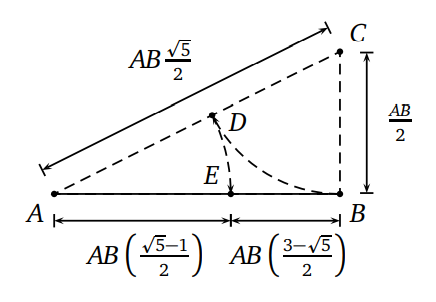
\includegraphics[width=0.5\linewidth]{book1} 

}

\caption{Ubicación de la sección aurea}\label{fig:aureo1}
\end{figure}

\hypertarget{propiedades-del-nuxfamero}{%
\subsection{Propiedades del número}\label{propiedades-del-nuxfamero}}

\hypertarget{nuxfamero-uxe1ureo-proporciuxf3n-uxe1urea-secciuxf3n-uxe1urea-aplicaciones}{%
\section{Número áureo, proporción áurea, sección áurea (Aplicaciones)}\label{nuxfamero-uxe1ureo-proporciuxf3n-uxe1urea-secciuxf3n-uxe1urea-aplicaciones}}

\hypertarget{rectuxe1ngulo-uxe1ureo-rectuxe1ngulos-uxe1ureos-y-composiciuxf3n}{%
\section{Rectángulo áureo (Rectángulos áureos) y composición}\label{rectuxe1ngulo-uxe1ureo-rectuxe1ngulos-uxe1ureos-y-composiciuxf3n}}

\hypertarget{sucesiones-de-fibonnacci-relacionado-con-el-nuxfamero-uxe1ureo}{%
\section{Sucesiones de Fibonnacci relacionado con el número áureo}\label{sucesiones-de-fibonnacci-relacionado-con-el-nuxfamero-uxe1ureo}}

La sucecion de Fibonnacci es la sucecion de numeros entros postivos
\[F=S_n={1,1,2,3,5,8,13,21,34, \ldots}\]

\hypertarget{rectuxe1ngulos-dinuxe1micos}{%
\section{Rectángulos dinámicos}\label{rectuxe1ngulos-dinuxe1micos}}

\hypertarget{pentuxe1gono-y-triuxe1ngulo-uxe1ureo-composiciuxf3n.}{%
\section{Pentágono y triángulo áureo (Composición).}\label{pentuxe1gono-y-triuxe1ngulo-uxe1ureo-composiciuxf3n.}}

\hypertarget{el-dodecaedro-construcciuxf3n-y-la-relaciuxf3n-con-el-nuxfamero-uxe1ureo}{%
\section{El dodecaedro construcción y la relación con el número áureo}\label{el-dodecaedro-construcciuxf3n-y-la-relaciuxf3n-con-el-nuxfamero-uxe1ureo}}

\hypertarget{el-icosaedro-construcciuxf3n-y-la-relaciuxf3n-con-el-nuxfamero-uxe1ureo}{%
\section{El icosaedro construcción y la relación con el número áureo}\label{el-icosaedro-construcciuxf3n-y-la-relaciuxf3n-con-el-nuxfamero-uxe1ureo}}

\hypertarget{proporciuxf3n-uxe1urea-de-la-figura-humana}{%
\section{Proporción áurea de la figura humana}\label{proporciuxf3n-uxe1urea-de-la-figura-humana}}

\hypertarget{fractales-sobre-el-conjunto-de-los-nuxfameros-complejos-y-cuaterniones}{%
\chapter{Fractales sobre el conjunto de los números complejos y cuaterniones}\label{fractales-sobre-el-conjunto-de-los-nuxfameros-complejos-y-cuaterniones}}

\hypertarget{nuxfameros-complejos.}{%
\section{Números complejos.}\label{nuxfameros-complejos.}}

\hypertarget{operaciones-con-nuxfameros-complejos}{%
\section{Operaciones con números complejos}\label{operaciones-con-nuxfameros-complejos}}

\begin{figure}

{\centering 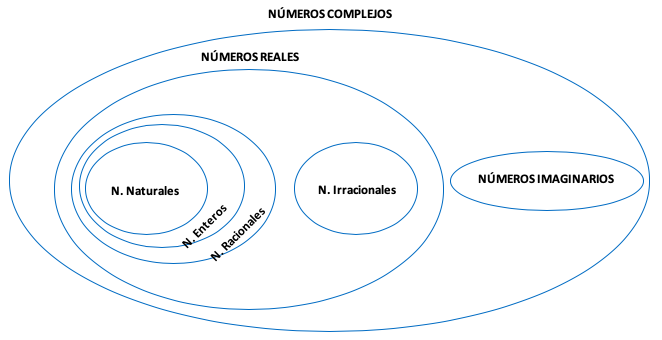
\includegraphics[width=1\linewidth,height=1\textheight]{complex} 

}

\caption{Esquema de los números complejos}\label{fig:complex}
\end{figure}

\hypertarget{funciones-en-el-plano-complejo-y-fractales-fz-zinmathbbc-cualesquiera}{%
\section{\texorpdfstring{Funciones en el plano complejo y fractales (\(f(z), z\in\mathbb{C}\) cualesquiera)}{Funciones en el plano complejo y fractales (f(z), z\textbackslash in\textbackslash mathbb\{C\} cualesquiera)}}\label{funciones-en-el-plano-complejo-y-fractales-fz-zinmathbbc-cualesquiera}}

\hypertarget{los-conjuntos-de-mandelbrot-fzz2c}{%
\section{\texorpdfstring{Los conjuntos de Mandelbrot (\(f(z)=z^2+c\))}{Los conjuntos de Mandelbrot (f(z)=z\^{}2+c)}}\label{los-conjuntos-de-mandelbrot-fzz2c}}

\hypertarget{los-conjuntos-de-julia-fzz2c}{%
\section{\texorpdfstring{Los conjuntos de Julia (\(f(z)=z^2+c\))}{Los conjuntos de Julia (f(z)=z\^{}2+c)}}\label{los-conjuntos-de-julia-fzz2c}}

\hypertarget{los-cuaterniones-y-conjuntos-de-mandelbrot-y-julia-3d-fractales-orguxe1nicos}{%
\section{Los cuaterniones y conjuntos de Mandelbrot y Julia 3D (Fractales orgánicos)}\label{los-cuaterniones-y-conjuntos-de-mandelbrot-y-julia-3d-fractales-orguxe1nicos}}

\hypertarget{reconocimiento-de-fractales-sobre-formas-orguxe1nicas}{%
\section{Reconocimiento de fractales sobre formas orgánicas}\label{reconocimiento-de-fractales-sobre-formas-orguxe1nicas}}

\hypertarget{sustentaciuxf3n-de-trabajos-1}{%
\section{\texorpdfstring{Sustentación de trabajos (\emph{Construcción de un fractal orgánico})}{Sustentación de trabajos ()}}\label{sustentaciuxf3n-de-trabajos-1}}

El número de oro \index{número de oro} es un número presente en la naturaleza, todo lo creado esta asociado con este número. La manera de recurrencia de las partes de los objetos visualmente atractivos están dispuestas de acuerdo a la razón y proporción del número áureo.

\begin{definition}[Numero áureo]
\protect\hypertarget{def:aureo}{}\label{def:aureo}Es un numero
\end{definition}

establecido por \(\frac{1+\sqrt{5}}{2}=1.618\) denotado por \(\phi\) o \(\Phi\) es decir \[\phi=\frac{1+\sqrt{5}}{2}=1.618\]

Además la inversa de este numero es \[\phi^{-1}=\frac{1}{\phi}=\frac{\sqrt{5}-1}{2}=0.618\]

\hypertarget{secciuxf3n-uxe1urea}{%
\section{Sección áurea}\label{secciuxf3n-uxe1urea}}

Es el proceso de generar el numero mediante el uso de una linea y la división que se realiza sobre este. Es decir dado un segmento \(AB\), un punto \(C\) uubicada entre los extremos \(A\) y \(B\) es la correspondiente (coloquialmente suele aproximarse con la tercera parte parte de este segmento). Exactamente se obtiene de la siguente manera. La razón de la \emph{longitud de todo el segmento} y la \emph{longitud del segmento mayor} es \textbf{proporcional} a la razón de la \emph{longitud del segmento mayor} sobre la \emph{longitud del segmento menor es decir}

\[
\frac{x+y}{x}=\frac{x}{y} \label{eq:aureo}
\]

simplificando \[
xy+y^2=x^2 \label{eq:new}
\] es posible hallar el valor de uno de ellos fijando la otra, sea por ejemplo \(y=2\) entonces la ecuación \eqref{eq:new} se reduce a \[
2x+4=x^2\Longleftrightarrow x^2-2x-4=0
\]

cuyas soluciones son \(x_1=2\frac{1+\sqrt{5}}{2}\) y \(x_2=2\frac{1-\sqrt{5}}{2}\)

en general si \(y=r\) entonces a ecuación \eqref{eq:new} se reduce a \[
rx+r^2=x^2\Longleftrightarrow x^2-rx-r^2=0
\]

cuyas soluciones son \(x_1=r\frac{1+\sqrt{5}}{2}=r\phi\) y \(x_2=r\frac{1-\sqrt{5}}{2}=r\left(-\frac{-1+\sqrt{5}}{2}\right)=r\left(-\frac{1}{\phi}\right)\)

\begin{remark}
La proporción (\ref(eq:aureo) es igual a una constante de prorpocionalidad que es igual a \(\phi\) es decir \(\frac{x+y}{x}=\frac{x}{y}=\phi\)
\end{remark}

\begin{figure}

{\centering 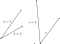
\includegraphics{proporcion} 

}

\caption{Circunferencia}\label{fig:C2}
\end{figure}

\hypertarget{rectuxe1ngulo-uxe1ureo}{%
\section{Rectángulo áureo}\label{rectuxe1ngulo-uxe1ureo}}

\hypertarget{pentuxe1gono-y-el-nuxfamero-de-oro}{%
\section{Pentágono y el número de oro}\label{pentuxe1gono-y-el-nuxfamero-de-oro}}

\hypertarget{dodecaedro-y-el-nuxfamero-de-oro}{%
\section{Dodecaedro y el número de oro}\label{dodecaedro-y-el-nuxfamero-de-oro}}

\hypertarget{aplicaciones-del-nuxfamero-de-oro}{%
\section{Aplicaciones del número de oro}\label{aplicaciones-del-nuxfamero-de-oro}}

\hypertarget{terminologuxedas}{%
\subsection{Terminologías}\label{terminologuxedas}}

Algunos de estos son:
\#\#\#\#\# El número de oro
\[\phi=1.618\]
\#\#\#\#\# La sección áurea
Es un punto, recta o plano que secciona una cantidad (Todo) de modo las partes que generan gurdan relación con el número de oro.

\textbf{\emph{``La razon del todo sobre la parte mayor es igual a la razon de la parte mayor sobre la parte menor''}}

Genera una ecuacion de segundo grado cuyas raices son \(\phi\) y \(\frac{1}{\phi}\)

\hypertarget{la-proporciuxf3n-uxe1urea}{%
\paragraph{La proporción áurea}\label{la-proporciuxf3n-uxe1urea}}

Es la igualdad de dos razones \[\frac{a}{b}=\frac{c}{d}=\phi=1.618\]
\#\#\#\#\# La sucesión áurea

1, \(\phi\), \(\phi^2\), \(\phi^3\). \(\ldots\)

\hypertarget{la-sucesion-de-fibonacci}{%
\paragraph{La sucesion de Fibonacci}\label{la-sucesion-de-fibonacci}}

2, 3, 5, 8, 13, 21, 34, 55, 89, 144, 233, 377, 610, 987, 1597, 2584, 4181, 6765, 10946, 17711, 28657, 46368, 75025, 121393, 196418, 317811, \ldots{}

si \(a_n\) es n termino geenral de la sucecion de Fibonnacci entonces
\[ \lim_{n \to \infty} \frac{a_n}{a_{n-1}}=\phi  \]

\hypertarget{ejemplo-aplicativo}{%
\subsection{Ejemplo aplicativo}\label{ejemplo-aplicativo}}

\hypertarget{aplicaciones-de-los-fractales-en-composiciones-complejas}{%
\chapter{Aplicaciones de los fractales en composiciones complejas}\label{aplicaciones-de-los-fractales-en-composiciones-complejas}}

En este capítulo se estudiará que los \textbf{objetos artísticos} siempre se componen de una \textbf{estructura fractal}. Estos aspectos son poco considerados al aplicar los fractales en composiciones complejas. Que se realizan de manera implícita e intuitiva en campos abstracto-figurativas.

\hypertarget{secuencias-orguxe1nicas-bajo-transformaciones-topoluxf3gicas}{%
\section{Secuencias orgánicas bajo transformaciones topológicas}\label{secuencias-orguxe1nicas-bajo-transformaciones-topoluxf3gicas}}

Se sabe que en la construcción de fractales existen dos tipos de transformaciones, \emph{las elementales y las topológicas}. En esta sección trataremos sobre las \emph{transformaciones topológicas} con el objetivo de \emph{modificar las formas de los términos} de una secuencia de manera que cada termino que se suceda, mantenga en lo posible las \emph{formas de los términos adyacentes}. En relación con el estudio comparativo de los seres vivos se tiene la siguiente definición, lo cual tiene mucha relación con los objetivos de esta sección y los subsiguientes \citet{homology}.

\begin{definition}[Homología]
\protect\hypertarget{def:homologia}{}\label{def:homologia}La \textbf{homología} es la \emph{relación} que existe entre \emph{dos partes orgánicas diferentes} de \emph{dos organismos distintos} cuando sus determinantes genéticos tienen el mismo origen evolutivo.
\end{definition}

\begin{definition}[Homotopía]
\protect\hypertarget{def:homotopia}{}\label{def:homotopia}En topología, y más precisamente en topología algebraica, dos aplicaciones continuas de un espacio topológico en otro se dicen homótopas (del griego homos = mismo y topos = lugar) si una de ellas puede ``deformarse continuamente'' en la otra.
\end{definition}

\begin{figure}[!ht]

{\centering 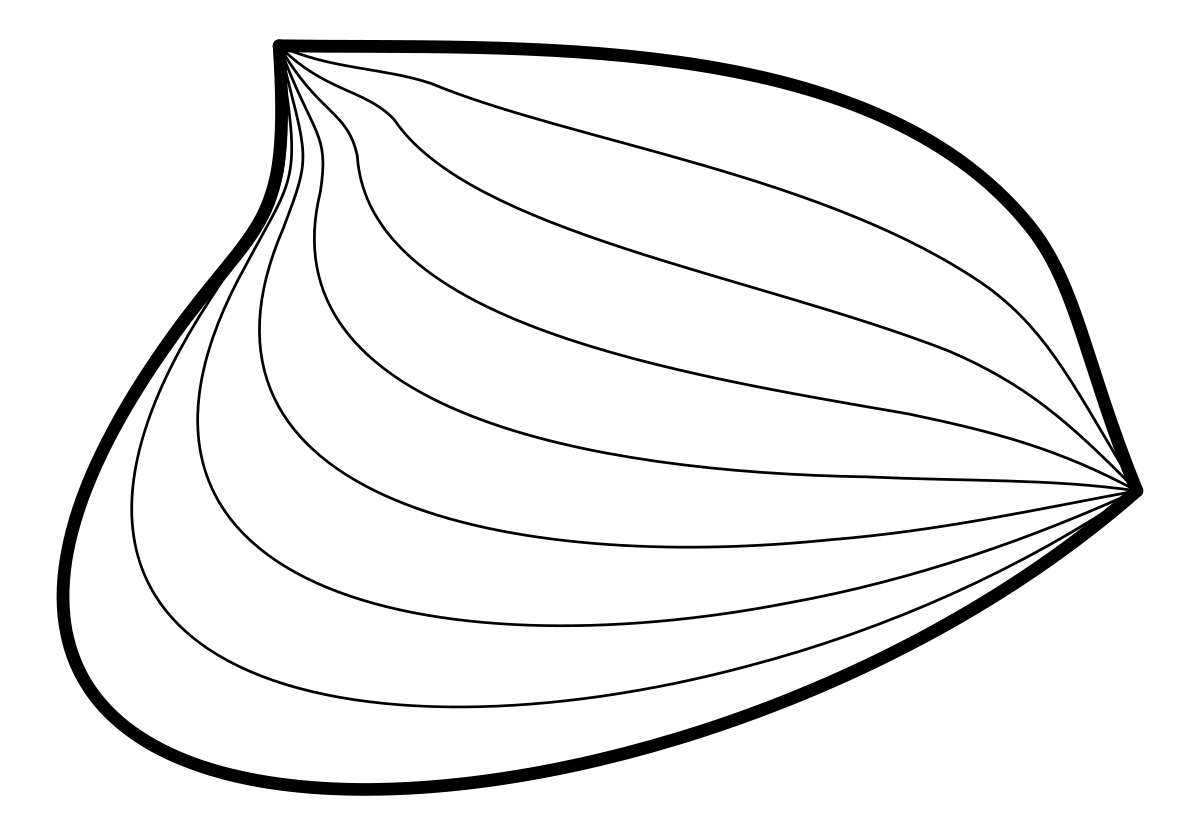
\includegraphics[width=0.5\linewidth]{homotopia} 

}

\caption{Los dos caminos en líneas punteadas que se muestran arriba son homótopos en relación a sus extremos. La animación muestra una posible homotopía entre ellos}\label{fig:homotopia}
\end{figure}

Como \citet{homology} comenta:

\begin{quote}
Existe homología entre órganos dados de dos especies diferentes, cuando ambos derivan del órgano correspondiente de su antepasado común, con independencia de cuán dispares puedan haber llegado a ser. Las cuatro extremidades pares de los vertebrados con mandíbula (gnatóstomos), desde los tiburones hasta las aves o los mamíferos, son homólogas. De la misma manera, el extremo de la pata de un caballo es homólogo al dedo mediano de la mano y el pie humano.
\end{quote}

\begin{remark}[Relación entre la homología y la sucesión bajo transformaciones topológicas]

Se observa que la \emph{homología} \index{homología} es una \emph{sucesión} de formas que mantiene \emph{similaridad} entre sus términos o elementos, es importante que la diferencia entre un termino y otro esta afectada por una ligera \textbf{transformación topológica}\index{transformación topológica}.

\end{remark}

En la observación anterior hace referencia de que todo los objetos de tipo secuencial, mantiene la homología.

\begin{figure}[!ht]

{\centering 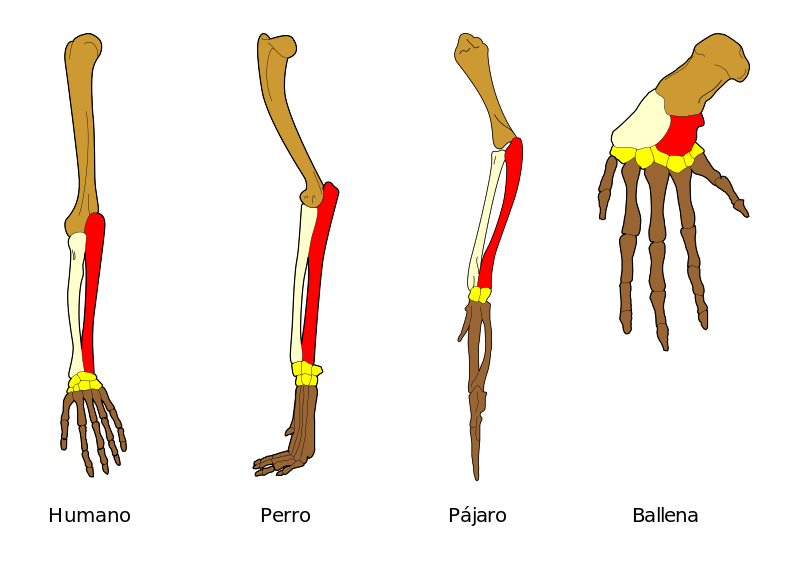
\includegraphics[width=1\linewidth]{homologia} 

}

\caption{Homología de varios huesos (mostrados en distintos colores) de las extremidades delanteras de cuatro vertebrados}\label{fig:homologia}
\end{figure}

\begin{figure}[!ht]

{\centering 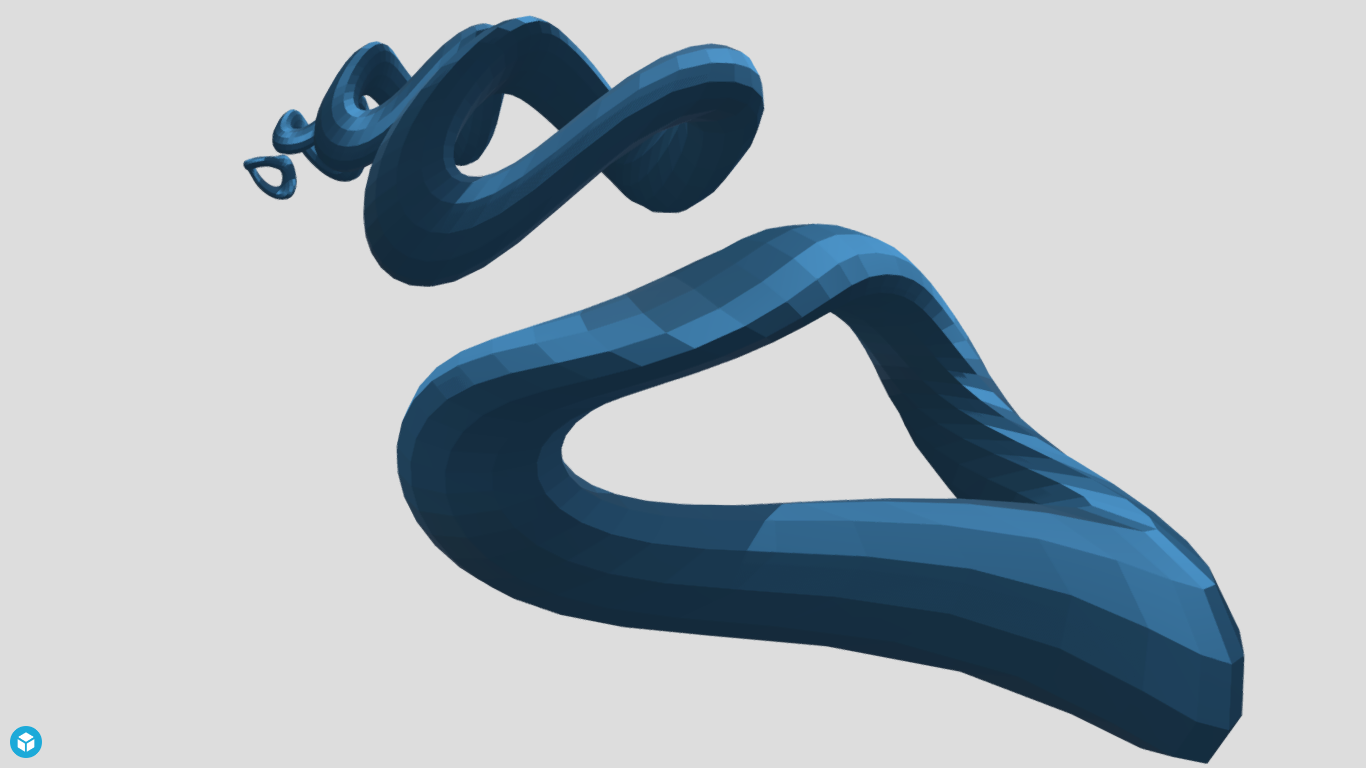
\includegraphics[width=1\linewidth]{sucecion} 

}

\caption{Sucesión orgánica bajo transformaciones topológicas}\label{fig:Suscecion}
\end{figure}

\hypertarget{fractales-orguxe1nicos-bajo-transformaciones-topoluxf3gicas-sketchfab-organic}{%
\section{Fractales orgánicos bajo transformaciones topológicas (Sketchfab organic)}\label{fractales-orguxe1nicos-bajo-transformaciones-topoluxf3gicas-sketchfab-organic}}

Se sabe que un fractal es una colección de sucesiones cuyos términos se constituyen de secuencias de formas homólogas. Es decir \emph{una secesión de sucesiones} por tanto esas formas que componen son copias transformadas topológicamente.

\begin{figure}[!ht]

{\centering 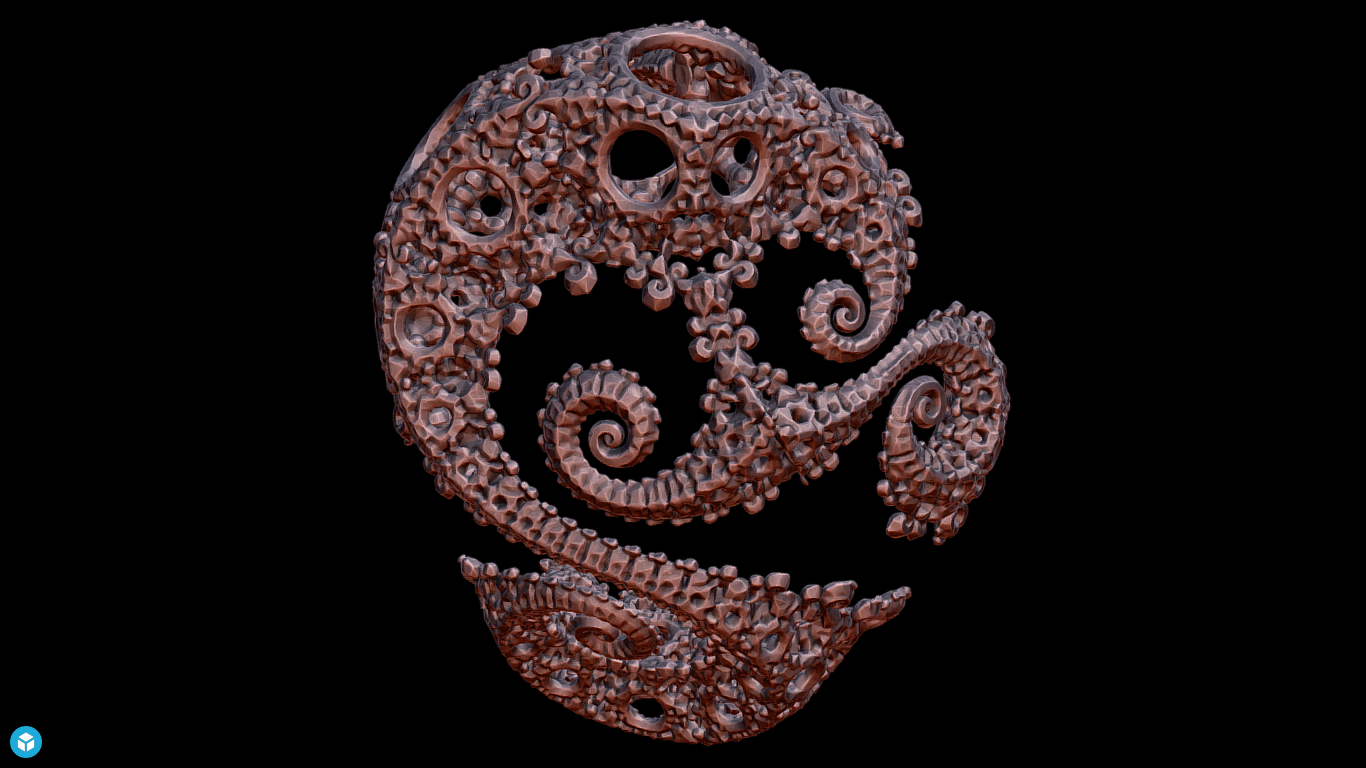
\includegraphics[width=1\linewidth]{Sketch} 

}

\caption{Fractales orgánicos bajo transformaciones topológicas - Sketchfab organic}\label{fig:Sketch}
\end{figure}

En l Figura \ref{fig:Sketch} se tiene la forma espiralada se sucede de acuerdo a la transformación topológica en cada uno de los términos.

\begin{figure}[!ht]

{\centering 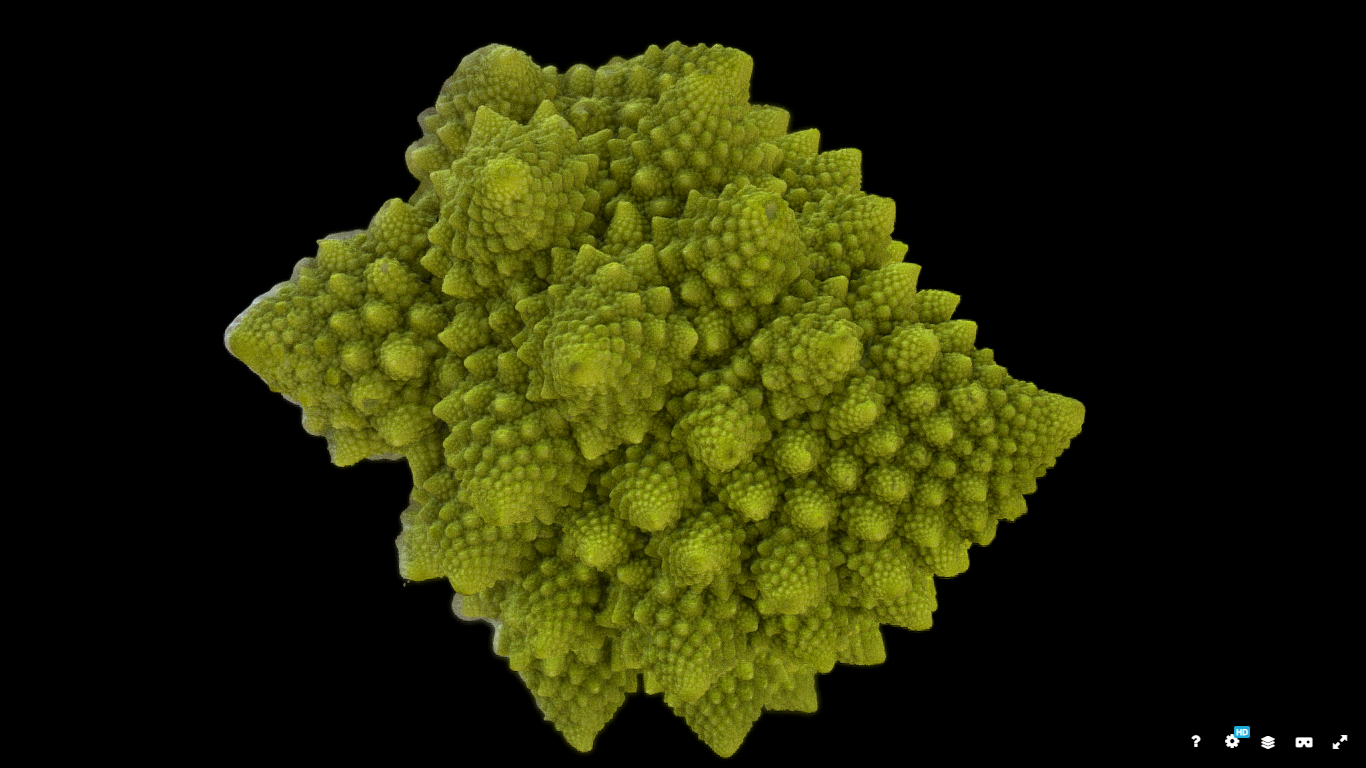
\includegraphics[width=1\linewidth]{Sketch2} 

}

\caption{Fractales orgánicos bajo transformaciones topológicas - Sketchfab organic}\label{fig:Sketch2}
\end{figure}

\hypertarget{la-figura-humana-como-un-fractal-fractal-body-modelado}{%
\section{La figura humana como un fractal (fractal body modelado)}\label{la-figura-humana-como-un-fractal-fractal-body-modelado}}

La figura humana se estructura en base a una suceción de estructuras fractales desde los niveleres moleculares, celulares, orgánicos, sistemáticos y corporales. Pues debido a ese orden se sucede la existencia humana. En este caso el arte se encarga de estudiar esos patrones a nivel corporal o físico de la figura humana. De acuerdo a las figura \ref{fig:body} y los subsiguientes se pone de manifiesto estructuras fractales, es decir secuencia de secuencias.

\href{https://www.behance.net/gallery/11339339/FRACTAL-BODY}{Body fractal}

\begin{figure}[!ht]

{\centering 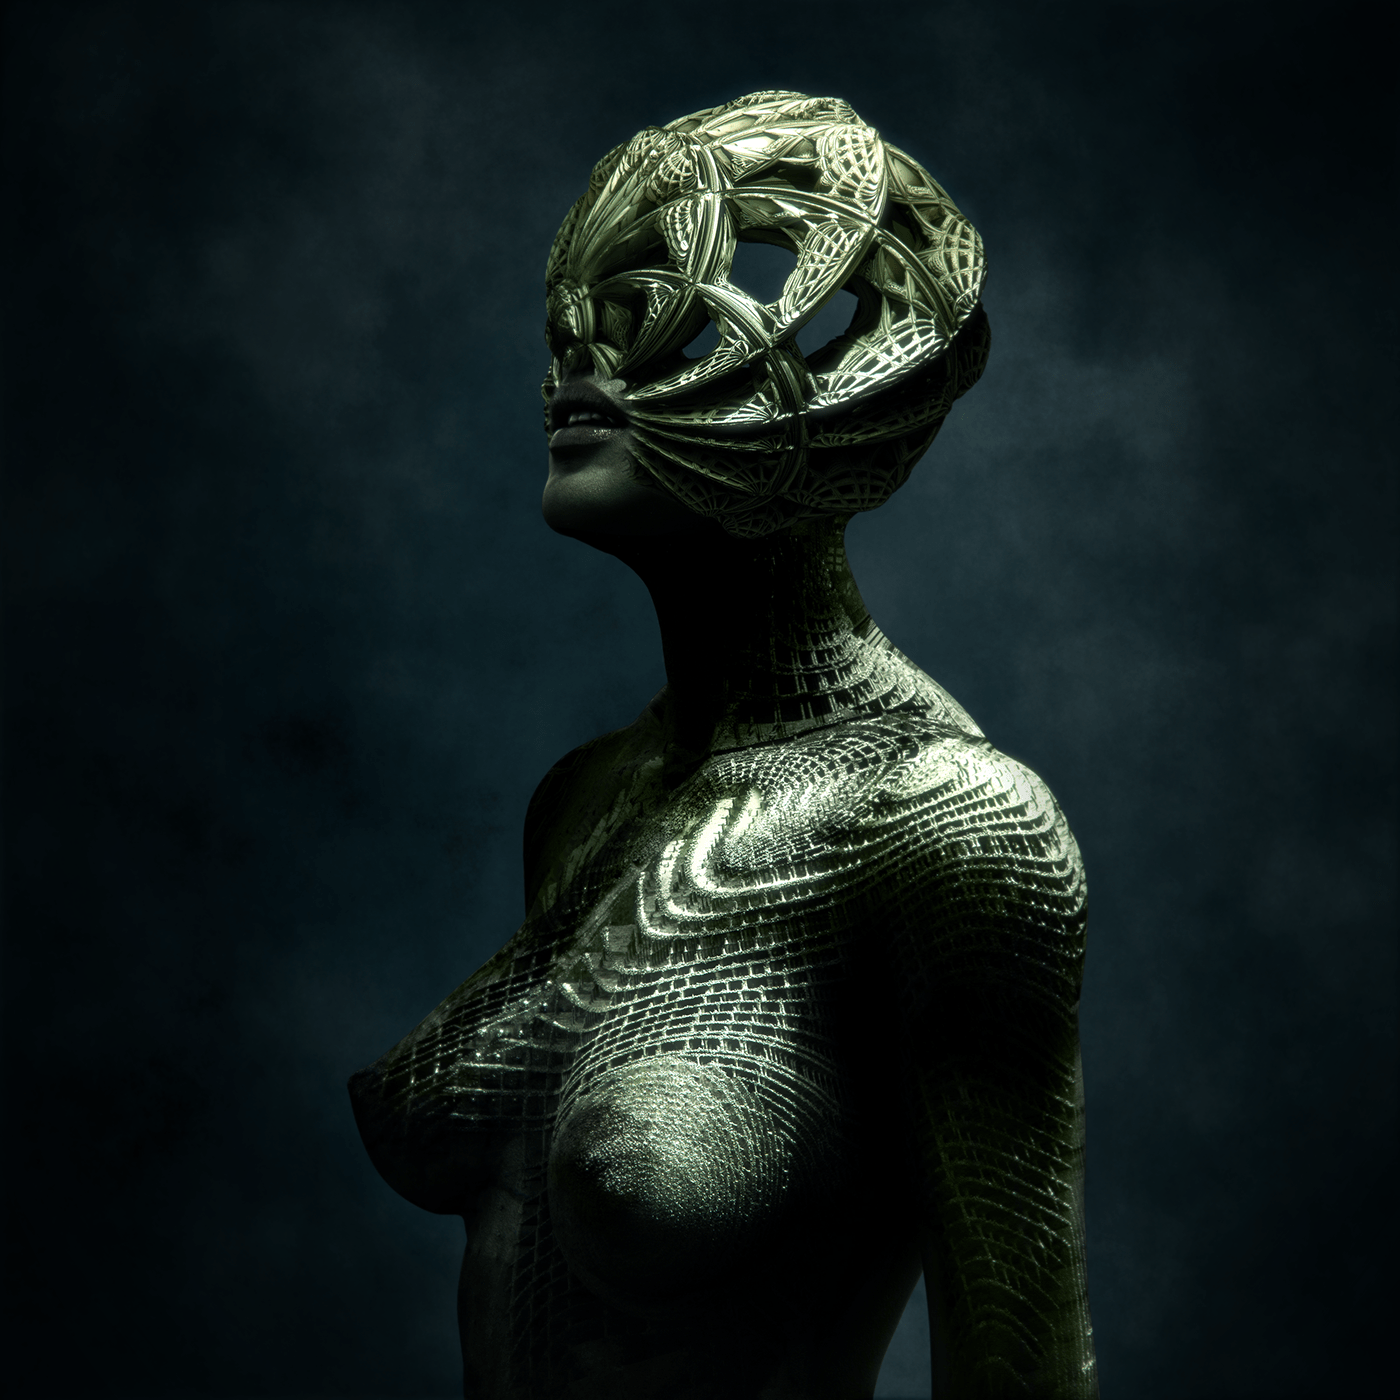
\includegraphics[width=0.7\linewidth]{body1} 

}

\caption{Construccion de la figura humana manifestando fractal}\label{fig:body1}
\end{figure}

\begin{figure}[!ht]

{\centering 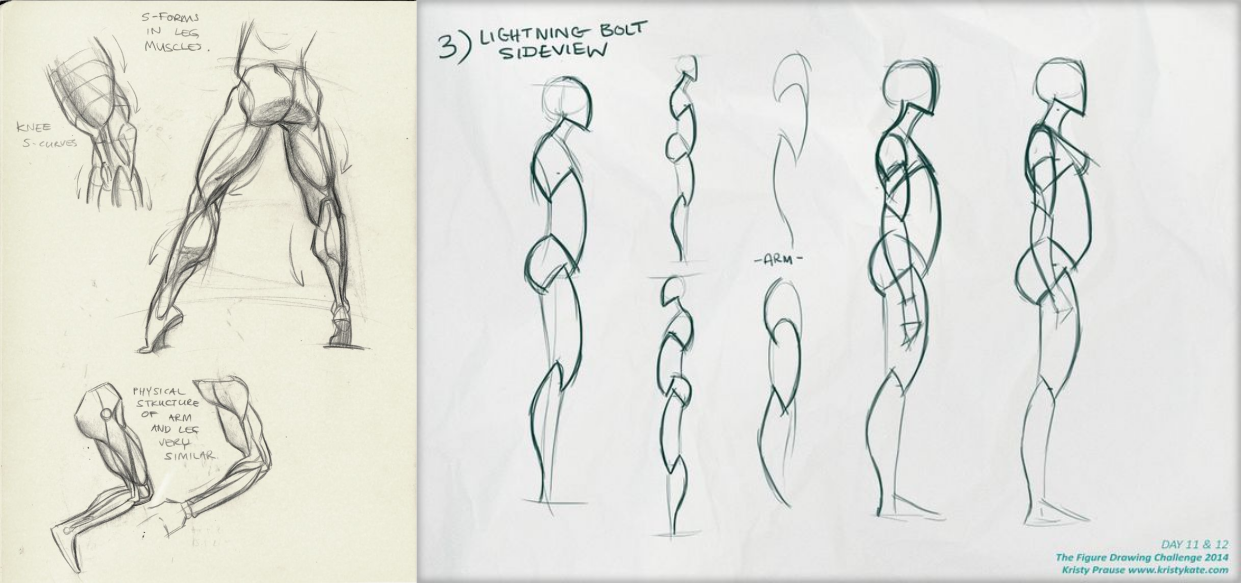
\includegraphics[width=1\linewidth]{body} 

}

\caption{Los ejes de la figura humana se suceden de acuerdo a la secuencia de segmentos de curvas y curvaturas de estas}\label{fig:body}
\end{figure}
\begin{figure}[!ht]

{\centering 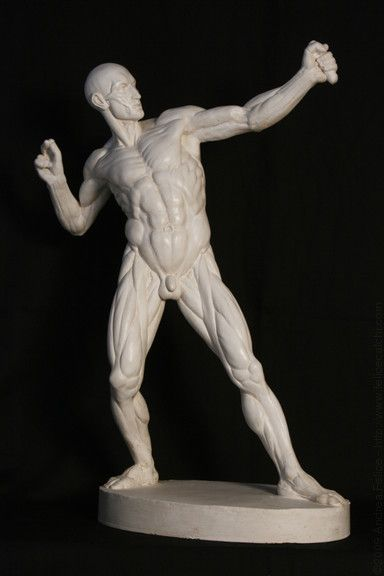
\includegraphics[width=1\linewidth]{body2} 

}

\caption{La estructura de la figura se sucede de acuerdo a una secuencia, además las protuberencias de los músculos son una coleccion de secuencias (fractal)}\label{fig:body2}
\end{figure}

\hypertarget{fractal-en-el-canon}{%
\section{Fractal en el canon}\label{fractal-en-el-canon}}

\hypertarget{softwares-generadores-de-fractales-2d-y-3d}{%
\section{Software's generadores de Fractales 2D y 3D}\label{softwares-generadores-de-fractales-2d-y-3d}}

\hypertarget{pov-ray-3d}{%
\subsection{POV-Ray (3D)}\label{pov-ray-3d}}

La persistencia de Vision Raytracer es una herramienta de software libre de alta calidad para crear impresionantes gráficos tridimensionales . El código fuente está disponible para aquellos que quieran hacer sus propios puertos.

\begin{figure}[!ht]

{\centering 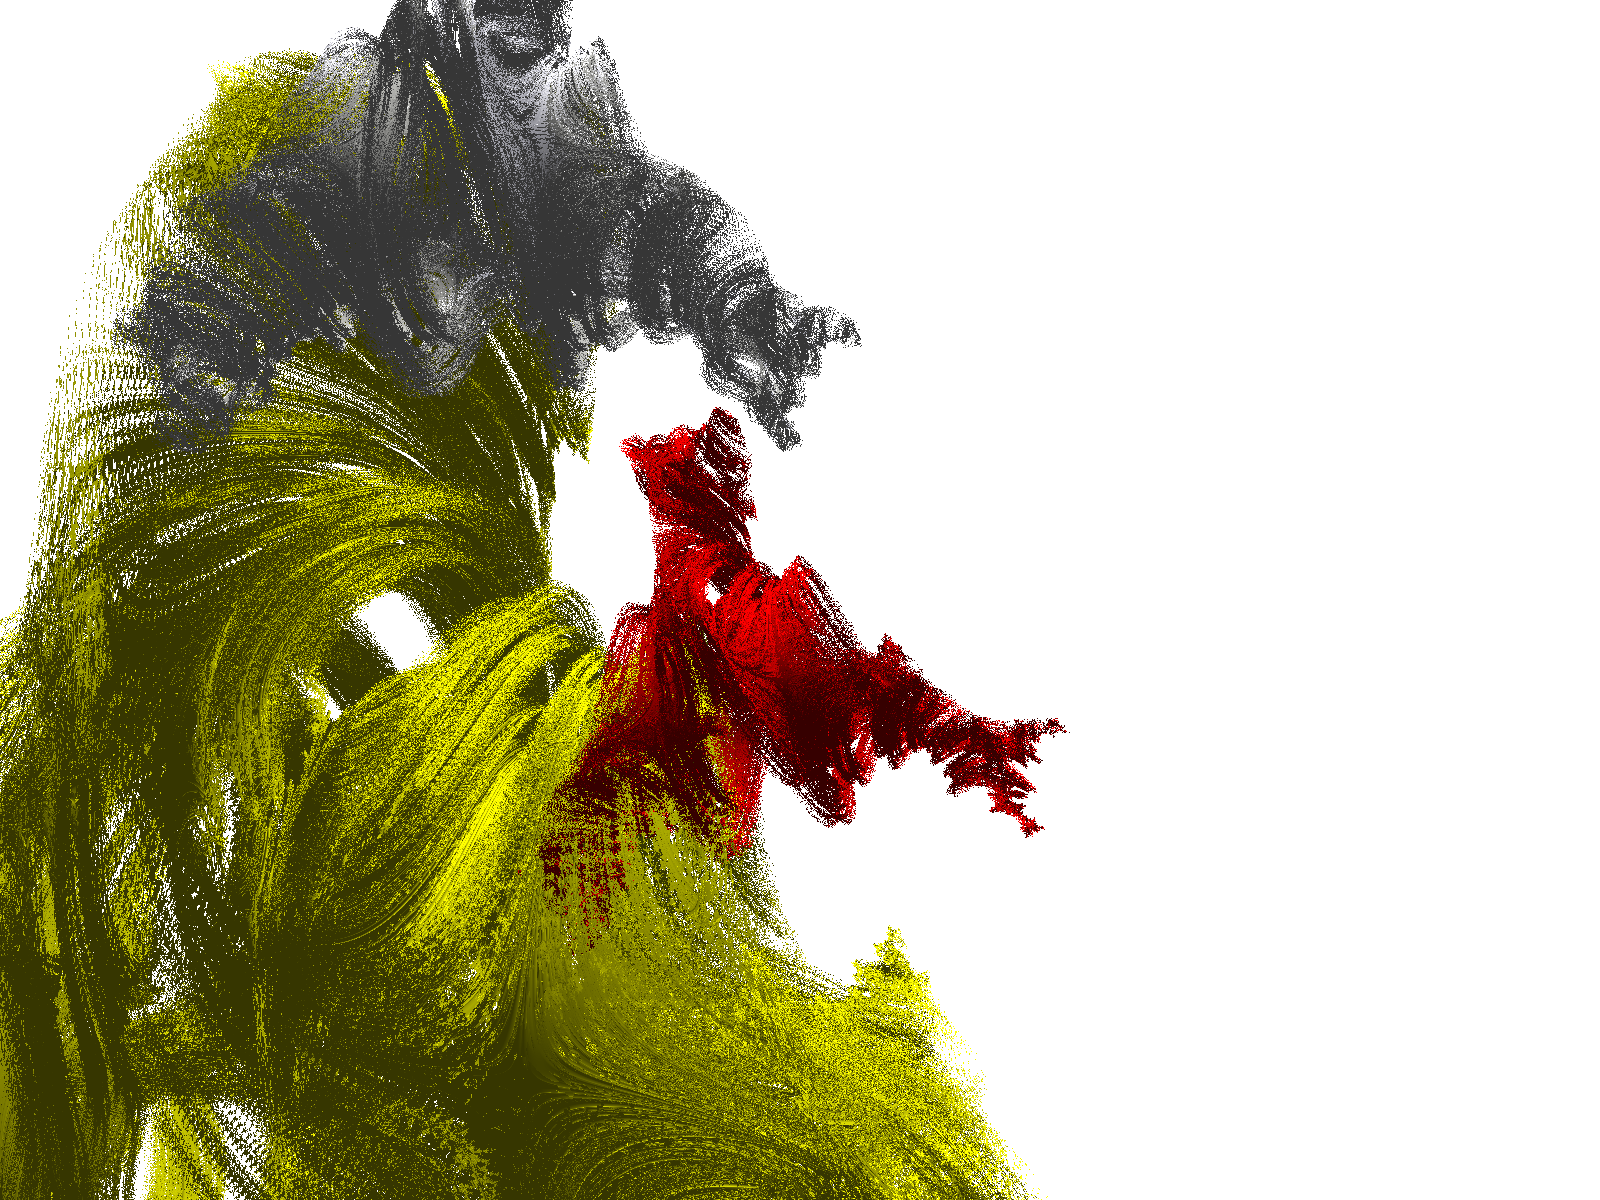
\includegraphics[width=1\linewidth]{povray} 

}

\caption{Homología de varios huesos (mostrados en distintos colores) de las extremidades delanteras de cuatro vertebrados}\label{fig:ray}
\end{figure}

\begin{Shaded}
\begin{Highlighting}[]
\NormalTok{\#version 3.6;}
\NormalTok{global\_settings\{ assumed\_gamma 1.3 max\_trace\_level 50\}}
\NormalTok{\#include "colors.inc"}
\NormalTok{\#include "functions.inc"}
\NormalTok{\#include "logo.inc"}

\NormalTok{background \{ color White \}}
\NormalTok{camera\{ location  \textless{}1,{-}2,{-}1\textgreater{}  }
\NormalTok{        angle 0 // direction 2*z}
\NormalTok{        right    x*image\_width/image\_height}
\NormalTok{        // keep propotions with any aspect ratio}
\NormalTok{        look\_at   \textless{}1,{-}.4,0\textgreater{}}
\NormalTok{      \}}
\NormalTok{light\_source \{\textless{}{-}140,200, 300\textgreater{}}
\NormalTok{   rgb \textless{}1.0, 1.0, 0.95\textgreater{}*1.5 \}}
\NormalTok{light\_source \{\textless{}{-}140,200, {-}300\textgreater{}}
\NormalTok{   rgb \textless{}1.0, 1.0, 0.95\textgreater{}*1.5 shadowless\}}
\NormalTok{light\_source \{\textless{} 140,200,{-}300\textgreater{}}
\NormalTok{   rgb \textless{}0.9, 0.9, 1.00\textgreater{}*1.9 \}}

\NormalTok{julia\_fractal\{ \textless{}{-}0.023,0.8,{-}0.83,{-}0.095\textgreater{}}
\NormalTok{   quaternion // quaternion hypercomplex}
\NormalTok{   cube             // Types: sqr  cube}
\NormalTok{   max\_iteration 20}
\NormalTok{   precision 200     // 10...500}

\NormalTok{   texture\{}
\NormalTok{  //   pigment\{ color rgb\textless{}0.85,0.1,0.1\textgreater{}\}}
\NormalTok{    // finish \{ phong 1\}}
\NormalTok{     pigment \{White*0.8\}}
\NormalTok{     //finish \{phong 0.7 reflection 0.1\}}
\NormalTok{     //normal \{bumps 0.05 scale 1\}}

\NormalTok{   \} // end of texture}
\NormalTok{   scale\textless{}.5,.5,.5\textgreater{}}
\NormalTok{   rotate\textless{}0,0,0\textgreater{}}
\NormalTok{   translate\textless{}0.5,0,{-}0.5\textgreater{}}
\NormalTok{\} // end of julia\_fractal {-}{-}{-}{-}{-}{-}{-}{-}{-}{-}}

\NormalTok{    julia\_fractal\{ \textless{}{-}0.023,0.8,{-}0.83,{-}0.095\textgreater{}}
\NormalTok{   quaternion // quaternion hypercomplex}
\NormalTok{   cube             // Types: sqr  cube}
\NormalTok{   max\_iteration 20}
\NormalTok{   precision 200     // 10...500}

\NormalTok{   texture\{}
\NormalTok{  //   pigment\{ color rgb\textless{}0.85,0.1,0.1\textgreater{}\}}
\NormalTok{    // finish \{ phong 1\}}
\NormalTok{     pigment \{Red*0.8\}}
\NormalTok{     //finish \{phong 0.7 reflection 0.1\}}
\NormalTok{     //normal \{bumps 0.05 scale 1\}}

\NormalTok{   \} // end of texture}
\NormalTok{   scale\textless{}0.5,.5,.5\textgreater{}}
\NormalTok{   rotate\textless{}0,20,0\textgreater{}}
\NormalTok{   translate\textless{}0.9,0,0.5\textgreater{}}
\NormalTok{\} // end of julia\_fractal {-}{-}{-}{-}{-}{-}{-}{-}{-}{-}}

\NormalTok{    julia\_fractal\{ \textless{}{-}0.023,0.8,{-}0.83,{-}0.095\textgreater{}}
\NormalTok{   quaternion // quaternion hypercomplex}
\NormalTok{   cube             // Types: sqr  cube}
\NormalTok{   max\_iteration 20}
\NormalTok{   precision 200     // 10...500}

\NormalTok{   texture\{}
\NormalTok{  //   pigment\{ color rgb\textless{}0.85,0.1,0.1\textgreater{}\}}
\NormalTok{    // finish \{ phong 1\}}
\NormalTok{     pigment \{Yellow*0.8\}}
\NormalTok{     //finish \{phong 0.7 reflection 0.1\}}
\NormalTok{     //normal \{bumps 0.05 scale 1\}}

\NormalTok{   \} // end of texture}
\NormalTok{   scale\textless{}2,2,2\textgreater{}}
\NormalTok{   rotate\textless{}0,0,0\textgreater{}}
\NormalTok{   translate\textless{}0,0,1.5\textgreater{}}
\NormalTok{\} //}
\end{Highlighting}
\end{Shaded}

\hypertarget{mandelbulb-3d}{%
\subsection{Mandelbulb-3d}\label{mandelbulb-3d}}

Mandelbulb 3D es una aplicación de software libre creada para imágenes fractales en 3D. Desarrollado por Jesse y un grupo de colaboradores de Fractal Forums , basado en el trabajo Mandelbulb de Daniel White y Paul Nylander, MB3D formula docenas de ecuaciones no lineales en una asombrosa variedad de objetos fractales. El entorno de renderizado 3D incluye iluminación, color, especularidad, profundidad de campo, efectos de sombra y brillo; permitiendo al usuario un control fino sobre los efectos de imagen. \href{https://www.mandelbulb.com/2014/mandelbulb-3d-mb3d-fractal-rendering-software/}{mandelbulb-3d}.

\hypertarget{wwwwwwwww}{%
\subsection{Wwwwwwwww}\label{wwwwwwwww}}

\hypertarget{paisajes-urbanos-y-rurales-como-fractales-mandelbulber}{%
\section{Paisajes urbanos y rurales como fractales (Mandelbulber)}\label{paisajes-urbanos-y-rurales-como-fractales-mandelbulber}}

\hypertarget{composiciuxf3n-fractales-mixta}{%
\section{Composición fractales mixta}\label{composiciuxf3n-fractales-mixta}}

\hypertarget{exposiciuxf3n-de-trabajos}{%
\section{\texorpdfstring{Exposición de trabajos (\emph{Paisaje fractal 3d digital, animado})}{Exposición de trabajos ()}}\label{exposiciuxf3n-de-trabajos}}

\hypertarget{fractales}{%
\chapter{Fractales}\label{fractales}}

En este capitulo se trata de los \emph{objetos plasticos} de característica \textbf{\emph{secuencial y fraccionaria}}.

\begin{definition}[Fractales]
\protect\hypertarget{def:fractal}{}\label{def:fractal}Son objetos geometricos bidimensionales o tridimensionales cuya estructura esta compuesta por partes que son copias transformadas del objeto total.
\end{definition}

Las transformaciones aquí consideradas son aquellas que conservan en lo posible las propiedades originales del objeto, es decir las transformaciones son las elementales (Traslacion, Rotacion, Homotescia, Reflexión) y los morfismos (isomorfismo, homeomorfismo, isometria, etc).

\begin{example}
\protect\hypertarget{exm:unnamed-chunk-3}{}\label{exm:unnamed-chunk-3}En la naturaleza se peden observe muchos ejemplares tales como las nuves los horatlizas
\end{example}

\begin{figure}[!ht]

{\centering 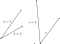
\includegraphics[width=1\linewidth]{proporcion} 

}

\caption{Hola}\label{fig:Doge}
\end{figure}

\begin{example}
\protect\hypertarget{exm:unnamed-chunk-4}{}\label{exm:unnamed-chunk-4}En la naturaleza se peden observe muchos ejemplares tales como las nuves los hortalizas, etc.
\end{example}

\hypertarget{fractales-bidimensionales}{%
\section{Fractales bidimensionales}\label{fractales-bidimensionales}}

\textbf{Copo de nieve de Koch}

\hypertarget{fractales-tridimensionales}{%
\section{Fractales tridimensionales}\label{fractales-tridimensionales}}

\hypertarget{nuxfameros-complejos}{%
\subsection{Números complejos}\label{nuxfameros-complejos}}

\begin{definition}[Conjuntos de Julia]
\protect\hypertarget{def:julia}{}\label{def:julia}Son conjuntos cuya forma bidimensionales o tridimensionales cuya estructura esta compuesta por partes que son copias transformadas del objeto total.
\end{definition}

\hypertarget{topologia-y-geometria-diferencial-de-las-formas}{%
\chapter{Topologia y geometria diferencial de las formas}\label{topologia-y-geometria-diferencial-de-las-formas}}

\citep{vincze2014college}

\hypertarget{ejercicios}{%
\section{Ejercicios}\label{ejercicios}}

\hypertarget{appendix-apendice}{%
\appendix \addcontentsline{toc}{chapter}{\appendixname}}


\hypertarget{intro}{%
\chapter{Proporción y canon}\label{intro}}

En todas las áreas del conocimiento humano se suele utilizar las razones y las proporciones ya sea de manera explicita o implícita por ejemplo en los laboratorios químicos, la gastronomía, la agricultura, la construcción, la arquitectura entre otros; en especifico en el arte. En este capitulo las cantidades involucradas serán las longitudes aunque se pueden relacionar incluso con cantidades de colores, cantidades de texturas, cantidad de sombras entre otros aspectos asociados al arte plástico. La importancia de las proporciones, es debido al manejo de cantidades diversas, manteniendo la relación de dos cantidades.

\hypertarget{razuxf3n}{%
\section{Razón}\label{razuxf3n}}

\begin{definition}[Razón]
\protect\hypertarget{def:razon}{}\label{def:razon}Una razón es una fracción de la forma

\[
\frac{a}{b}\label{eq:fraccion}
\]
\end{definition}

donde \(a\) y \(b\) son números reales la fracción \textbf{\emph{representa}} la relación que existe entre los números \(a\) y \(b\) es decir estas cantidades están asociadas.

En la ecuación \eqref{eq:fraccion} el resultado de dividir la fracción recibe el cociente, ademas \(a\) y \(b\) se denominan numerador y denominador respectivamente. Si \(a>b\) la fracción recibe el nombre e \emph{fracción propia} \index{fracción propia} y si \(a<b\) la fracción recibe el nombre e \emph{fracción impropia} \index{fracción impropia}

\hypertarget{proporciones}{%
\section{Proporciones}\label{proporciones}}

\begin{definition}[Proporcion]
\protect\hypertarget{def:proporcion}{}\label{def:proporcion}Una proporción es la igualdad de dos razones.

\[
\frac{a}{b}=\frac{c}{d}\label{eq:proporcion}
\]
\end{definition}

\begin{remark}[Observación]
En una proporción sucede que si \(a\) crece o decrece, \(b\) crece o decrece multiplicada con la misma cantidad; en este caso recibe el nombre de proporción directa y si \(a\) crece o decrece, \(b\) decrece y crece en este caso recibe el nombre proporción inversa. Generalmente en el arte plástico se utiliza las proporciones directas.
\end{remark}

\begin{example}[Ejemplo]
\protect\hypertarget{exm:wwwww}{}\label{exm:wwwww}Las fracciones \(\frac{a}{b}\) y \(\frac{c}{d}\) no son necesariamente iguales, generalmente esto significa conservar las cantidades \(a\) y \(b\) de manera proporcional es decir \(\frac{a}{b}=\frac{na}{nb}\) donde \(n\) es cualquier número real.
\end{example}

Las fracciones \(\frac{a}{b}\) y \(\frac{c}{d}\) no son necesariamente iguales, generalmente esto significa conservar las cantidades \(a\) y \(b\) de manera proporcional es decir \(\frac{a}{b}=\frac{na}{nb}\) donde \(n\) es cualquier número real.

Esta igualdad de fracciones (proporción) no ayuda a escalar (agrandar o reducir) cualquier figura 2d o 3d. Es decir si tenemos un modelo (linea poligonal izquierda en la Figura \ref{fig:ww1}), cuyas dos longitudes son \(a\) y \(b\), además en la copia a realizar, (linea poligonal de la derecha en la Figura \ref{fig:ww1}), establecemos la longitud \(c\) como la copia trasformada de la longitud \(a\) (un numero mayor a \(a\) si deseamos aumentar el tamaño con respecto al original y de manera inversa si deseamos reducir el tamaño); la longitud \(x\) es la incógnita que debe hallarse para mantener el tamaño de menera proporcional.

Si deseamos averiguar la longitud de \(x\) de manera proporcional asociado al valor \(c\) dado por conveniencia, primero se genera la razón \(\frac{a}{b}\) asociado al modelo y la razón \(\frac{c}{x}\) en la copia, en ese orden es decir \(c\) y \(a\) en el numerador pues \(c\) es la trasformación de \(a\) que se estableció

theorem Theorem thm
lemma Lemma lem
corollary Corollary cor
proposition Proposition prp
conjecture Conjecture cnj
definition Definition def
example Example exm
exercise Exercise exr
hypothesis Hypothesis hyp
\[
\frac{a}{b}=\frac{c}{x}\Longleftrightarrow ax=bc \Longleftrightarrow x=\frac{bc}{a}
\]

Sea \(a=3\), \(b=2\) y \(c=5\) en la figura \ref{fig:ww1} entonces\[
\frac{3}{2}=\frac{5}{x}\Longleftrightarrow 3x=2\cdot5 \Longleftrightarrow x=\frac{10}{3}=3.333
\]

\begin{figure}

{\centering 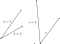
\includegraphics{proporcion} 

}

\caption{Proporción}\label{fig:ww1}
\end{figure}

Este proceso se puede iterar en una forma poligonal cuyo número de lados es mayor a dos, por ejemplo en la Figura \ref{fig:ww}, se tiene tres procesos adicionales estableciendo como punto partida al segmento \(GF\) luego se traza dos semirectas cuyo extremos coinciden con los extremos del segmento \(GF\), ademas es necesario conservar los ángulos de estos con respecto al segmento \(GF\) es decir \(\angle CBA=\angle FGK\) y \(\angle DCB=\angle IFG\). Entonces construimos los segmentos de longitud \(GK=GF\frac{AB}{BC}\) \(FI=GF\frac{CD}{BC}\) deducidas a partir de las proporciones

\[
\frac{GK}{GF}=\frac{AB}{BC}\: \text{ y }\: \frac{FI}{GF}=\frac{CD}{BC}
\]los extremos \(K\) e \(I\) deben estar sobre las semirectas correspondientes, finalmente se proporciona el segmento \(KH\) con el mismo procedimiento es decir ángulo \(\angle BAE=\angle GKH\) y longitud \(KH=KG\frac{EA}{BC}\)

\begin{figure}

{\centering 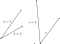
\includegraphics[width=1\linewidth,height=1\textheight]{proporcion} 

}

\caption{Proporción de un polígono}\label{fig:ww}
\end{figure}

Todo figura de la realidad se pueden inscribrir en un polígono por tanto puede se predispone a la proporción. Por ejemplo considere la Figura \ref{fig:ww} dada.

\hypertarget{canon}{%
\section{Canon}\label{canon}}

Debido a la poligonalización de las figuras en general es posible establecer un modelo cuyas subdivisión conlleve a un modelo aplicable en futuras representaciones.

::: \{.definition \$canon name=``Canon''\}
Las proporciones perfectas o ideales del cuerpo humano y alude a las relaciones armónicas entre las distintas partes de una figura.
:::

\begin{figure}

{\centering 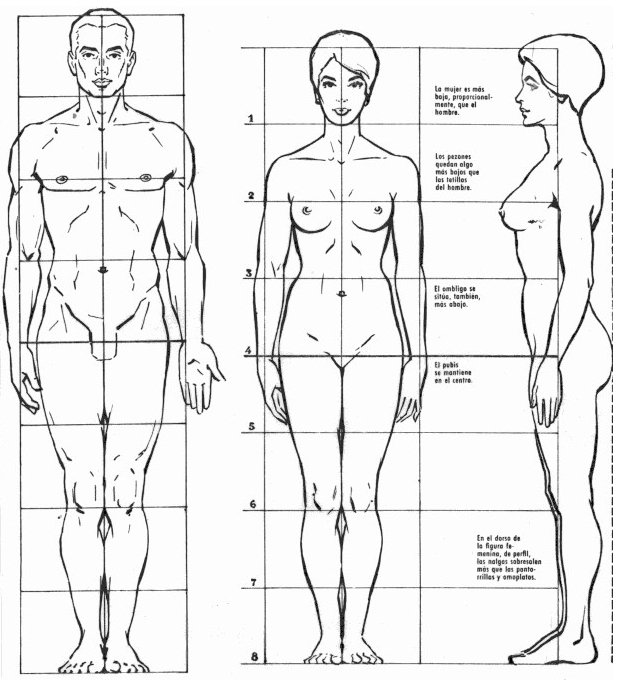
\includegraphics[width=1\linewidth,height=1\textheight]{canon} 

}

\caption{Proporción de un polígono}\label{fig:canonfig}
\end{figure}

\hypertarget{perspectiva-cuxf3nica}{%
\chapter{Perspectiva cónica}\label{perspectiva-cuxf3nica}}

\citep{xie2015}

\hypertarget{raices-de-una-ecuacion-de-segundo-grado}{%
\section{Raices de una ecuacion de segundo grado}\label{raices-de-una-ecuacion-de-segundo-grado}}

\hypertarget{propiedades-de-una-ecuacion-de-segundo-grado}{%
\section{Propiedades de una ecuacion de segundo grado}\label{propiedades-de-una-ecuacion-de-segundo-grado}}

\hypertarget{ecacuaciones-lineales-de-primer-grado}{%
\chapter{Ecacuaciones lineales de primer grado}\label{ecacuaciones-lineales-de-primer-grado}}

\hypertarget{soluciones-de-ecuacuiones-lineales-de-primer-grado}{%
\section{Soluciones de ecuacuiones lineales de primer grado}\label{soluciones-de-ecuacuiones-lineales-de-primer-grado}}

\hypertarget{soluciones}{%
\section{Soluciones \ldots{}}\label{soluciones}}

\hypertarget{forma-matricial-de-una-ecuaciuxf3n-lineal}{%
\section{Forma matricial de una ecuación lineal}\label{forma-matricial-de-una-ecuaciuxf3n-lineal}}

  \bibliography{book.bib}

\printindex

\end{document}
